\documentclass[12pt]{article}
\usepackage[utf8x]{inputenc}
\usepackage[T1]{fontenc}
\usepackage{import}
\usepackage[french]{babel}
\usepackage{import}
\usepackage{graphicx}

\title{Projet TDL : Compimlateur Micro Java}

\author{ Casanova Guillaume \\
	\and 
	 Leroux Frédéric \\
	\and
	 Palandri Rémi
	}

\date{\today}
% Hint: \title{what ever}, \author{who care} and \date{when ever} could stand 
% before or after the \begin{document} command 
% BUT the \maketitle command MUST come AFTER the \begin{document} command! 
\begin{document}

\maketitle

\begin{abstract}

\end{abstract}

\newpage
\setcounter{tocdepth}{1} \tableofcontents

\newpage

\section{Les classes JAVA}
	
	\subsection{Diagramme UML}
		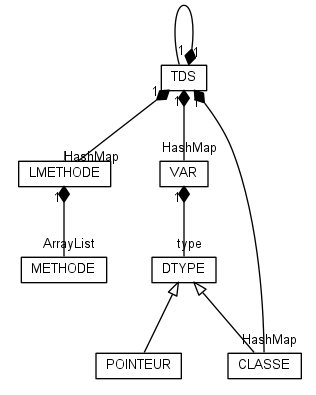
\includegraphics[width=10cm,height=88mm]{img/graph.png}
	\subsection{La TDS}
		
		\subimport{text/}{tds.tex}
\newpage
\section{Laison tardive}
		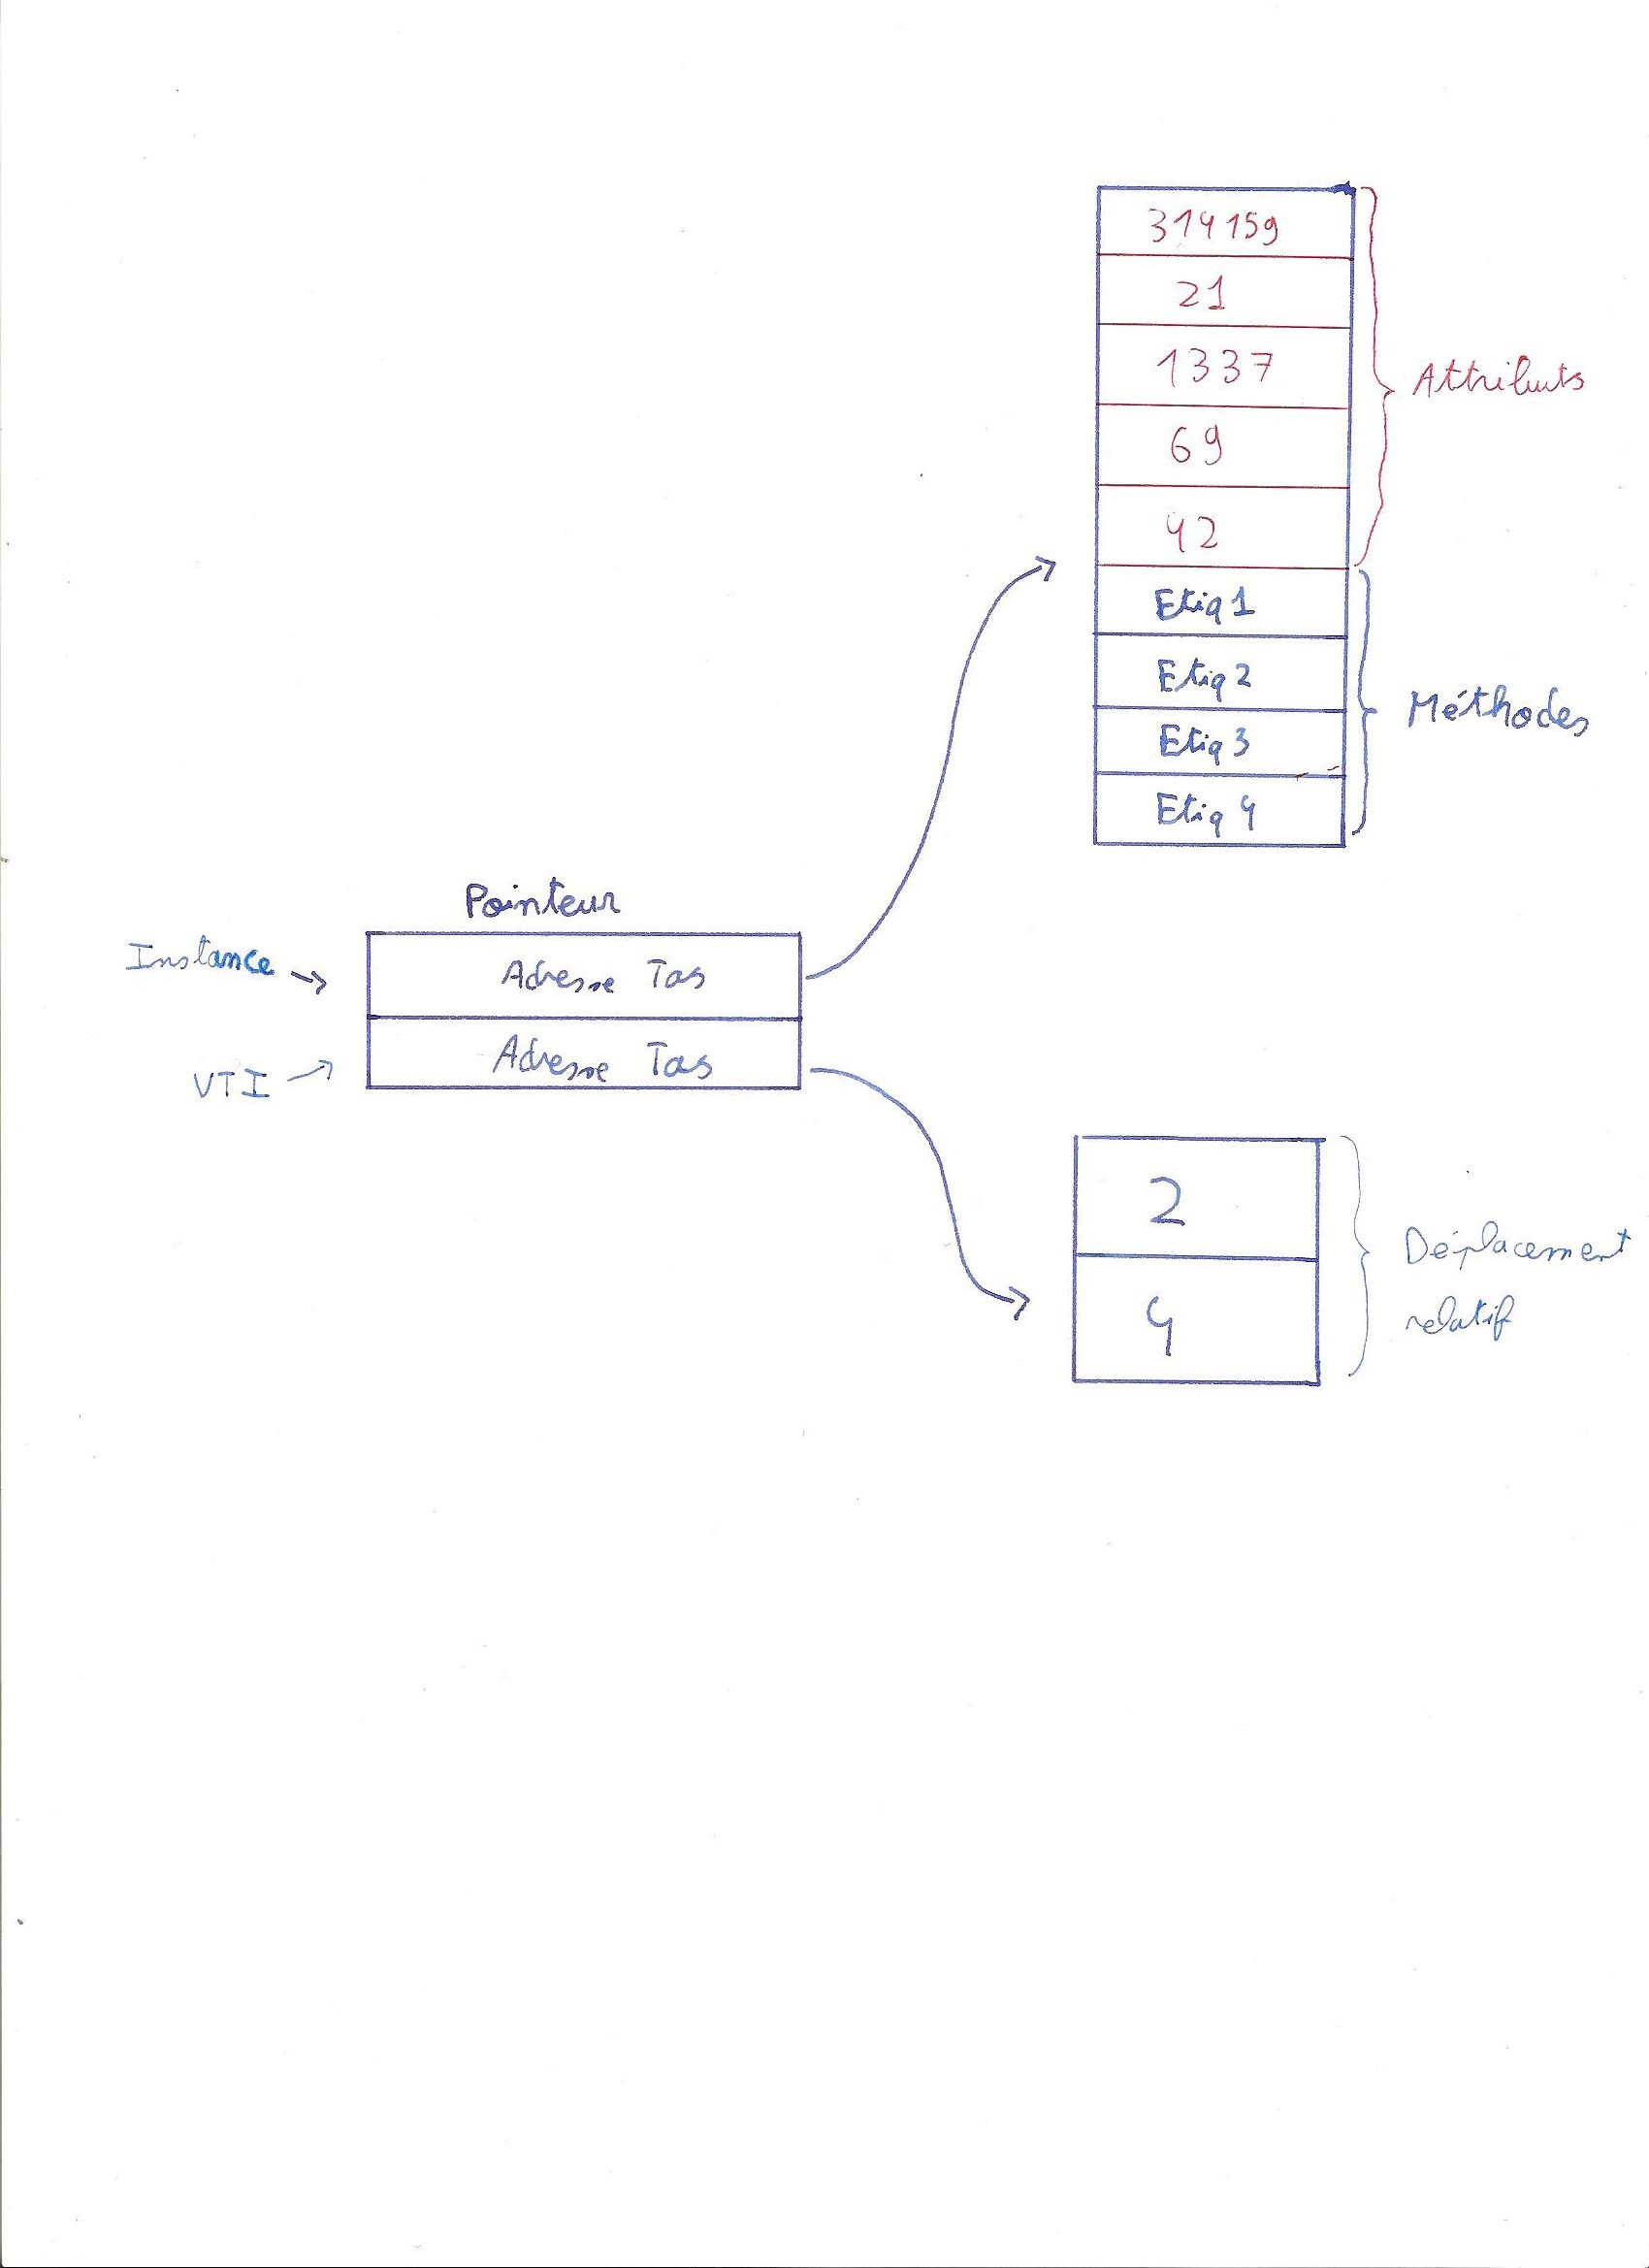
\includegraphics[width=10cm,height=90mm]{img/scan.jpeg}
		\subimport{text/}{tardive.tex}
\newpage
\section{Les trois passes}
		\subimport{text/}{trois-passes.tex}	
\newpage
\section{Problèmes principaux rencontrés}
 	\subsection{La surcharge}
		\subimport{text/}{problem-surcharge.tex}
	\subsection{Les règles E et ER}
		\subimport{text/}{problem-regle.tex}
\newpage
\section{Amélioration du code}

	\subsection{Le print}
		\subimport{text/}{print.tex}

	\subsection{Le this}
		\subimport{text/}{this.tex}
	\subsection{Le return}
		\subimport{text/}{return.tex}
%	\subsection{Le while}
%	\subsection{Le for}
\newpage
\section{Les tests}


\end{document}
